
\documentclass{article}

\usepackage{graphicx}
\usepackage{geometry}
\geometry{margin=1.5in}

\title{Predicting the United States Unemployment Rate}
\author{Orhan Koc \\
	University of Washington  \\
	\and 
	Kevin Chong  \\
	University of Washington  \\
	\and 
	Kristina Litau\\
	University of Washington  \\
	}
\date{\today}

\begin{document}
\maketitle


\begin{abstract}
	Unemployment rate (UR) is one of the most crucial metrics to convey the economic outlook of a country, affecting everyone on the socioeconomic spectrum. Effects of unemployment include a decrease in growth, capacity, individual purchasing power, and gross domestic product (GDP). Given this, accurately forecasting the UR has been a goal for many researchers and portfolio managers to gain an edge on the market. In this study, we will model UR using a data set comprised of macroeconomic metrics of the country being forecasted, UR of other countries, and retail food price data. We will use a variety of common methods in machine learning and compare the results with respect to the Root Mean Squared Error (RMSE) for each model. 
\end{abstract}

\newpage
\tableofcontents
\newpage

\section{Introduction}

	\subsection{Basic Setting}
	Unemployment Rate shows the inefficiencies of the economic system, or the maladjustment of the supply and demand of the labor market [1] which led to continuous attempts at forecasting by the academia and the industry. It’s important to realize UR for each industry can be derived from the cumulative UR prediction model, which is also a powerful tool in determining the growth and decline of job markets.

	Figure 1 shows the 70-year unemployment chart for the United States. Using this 70-year chart helps observe the cyclical nature of unemployment, which can help determine what approach to use. Another notable observation is that variation is not constant throughout the time window, which may suggest the function is heteroscedastic.

	\begin{center}
		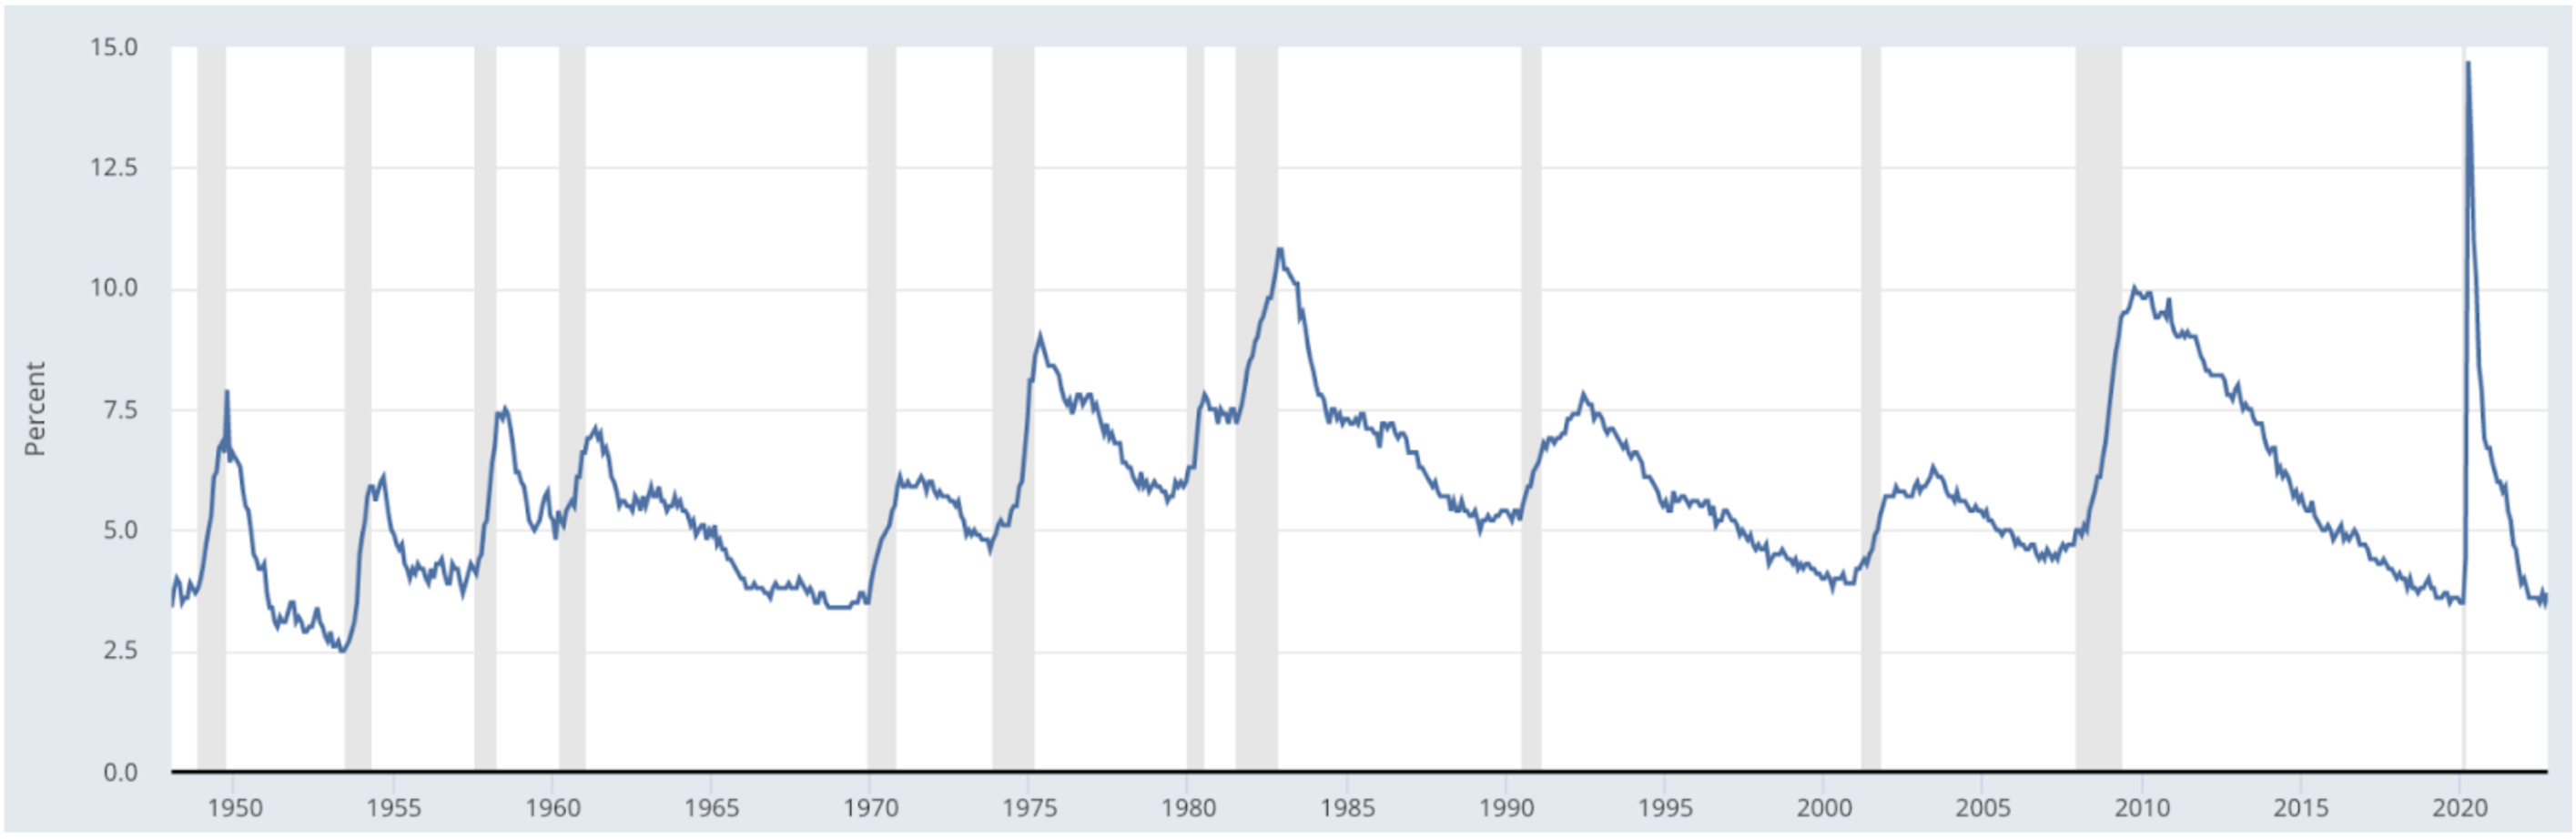
\includegraphics[width=1\textwidth]{assets/intro.png}
		\textit{Figure 1}
	\end{center}
	Our goal is to test the modeling accuracy (of the UR) using multiple machine learning methods: Linear regression, ARIMA, Decision Tree, and Random Forest. We will devise separate models using these methods and extrapolate for next year. After we have models at hand, we will conduct a Root Mean Squared Error analysis to determine which model is less wrong in modeling and forecast the future using the model.

	\subsection{Data}
	In devising our models, we will use 3 different data sets: Retail Food Price data, Macro Metrics, and the Unemployment Rate of foreign countries. The datasets are chosen based on a brainstorm conducted by the researchers with corresponding justifications stated below. An explanation of variable abbreviations is included in Appendix A, and sources for the aforementioned datasets are included in Appendix C.

	\textbf{Retail Food Prices} affect every individual due to basic needs, it is expected that higher prices will reduce purchasing power. A gross decrease in purchasing power is commonly handled (by the government) with an increase in the money supply. In 1958, William Phillips was the first economist to show the inverse relationship between unemployment and inflation [3], also known as the Phillips Curve, which is why we decided to include Retail Food Prices in our dataset.
	
	\textbf{Macro Metrics} cover a wide array of metrics that describe the economic outlook of a country. Our dataset covers metrics such as the Producers' Purchase Index (PPI), Customers' Purchase Index (CPI), Inflation, Median Household Income, et cetera. Many researchers have used the unemployment rate as a parameter to forecast the metrics described above, we entertain the idea that the relationship could be both ways.
	
	\textbf{Unemployment Rate of Foreign Countries} is an interesting idea to explore in light of a popular and somewhat controversial economic phenomenon known as the catch-up effect. The catch-up effect (also known as convergence theory) states that all economies will eventually converge in terms of per capita income. This hypothesis has been tested via various methods [4], but the results do not seem to entirely reject nor fail to reject the null hypothesis of convergence. We entertain the idea of convergence by including it in our dataset.
	
	It’s important to note even though we have a single dataset for all of the approaches mentioned below, each method uses a different subset of the dataset. In other words, each method has a different basis for forecasting UR - which isn’t the fairest setting to assess methods but will yield the most accurate forecast for each method. The reason for such an experiment setting is due to the nature of time series analysis, which requires the past values of the data being forecasted rather than a separate dataset (such as in Linear Regression based approaches).
	

	\subsection{Data Cleaning}
	We decided to combine multiple data sets to devise comparison models. To analyze data comprehensively for Linear Regression, Decision Tree, and Random Forest, we had to merge the datasets into one using mutual dimensions and granularity. Furthermore, for ARIMA, where we had to standardize the UR time series data. 

	After data cleaning, we split the UR dataset into two parts, each iteration, for testing and training purposes. The training subset is used to modify the model to fit new information. The testing subset is used to validate the devised model.
	
\section{Theory \& Model}
	For each method, we will state the justification of the chosen method, the method applicability to the chosen dataset, the theory of the method, and the implementation of the corresponding theory to build a model. Methods are sorted in such order that 3.1 Linear Regression is the basis for 3.2 ARIMA, and 3.3 Decision Tree is the basis for 3.4 Random Forest.
	
	\subsection{Linear Regression}
	Linear Regression builds a linear relationship between the independent variables (Dataset) and the dependent variable (Unemployment Rate) Every independent variable is assumed to have a linear effect on the dependent variable. This method measures the relevance of the desired parameters to decide whether a relationship exists.
	\begin{equation}
		y= \beta_0 + \sum_{i=1}^{p}(\beta_{i}x_i+\epsilon)
	\end{equation}
	The Linear Regression model was trained and tested by a combination of macro, retail food price and UR of other countries datasets. In order to prevent noise, instead of using the UR of individual countries, countries were grouped together based on location and political affiliations (The Organization for Economic Cooperation and Development, Group of 7, European Union, European Area). The findings are shown in Figure 2
	
	
	\begin{center}
		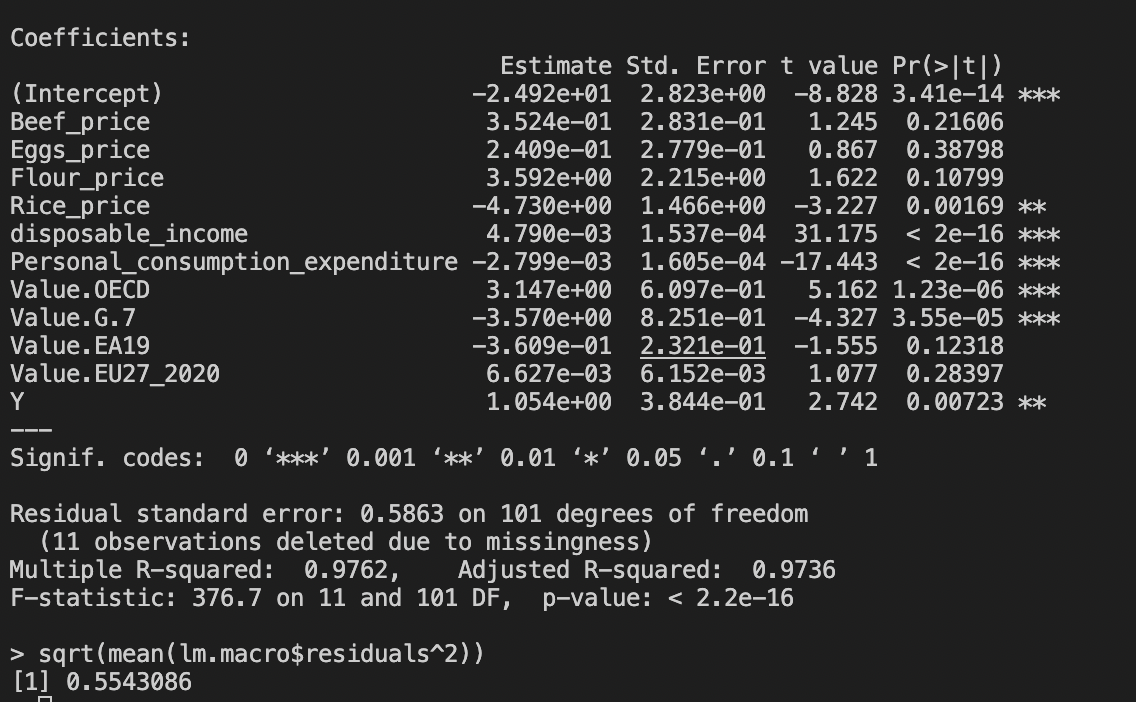
\includegraphics[width=1\textwidth]{assets/linReg.png}
		\textit{Figure 2}
	\end{center}
	The resulting model before ANOVA has an RMSE value of 0.5543. Looking at the $Pr(>|t|)$ column, we can 
	identify significant variables, such as Beef price, rice price, disposable income, OECD UR, EA19 UR and such.
	\subsection{ARIMA}
	The effects of unemployment and the causes of unemployment are surprisingly very similar, hinting at the presence of a feedback loop. This observation may indicate unemployment rate is inherently cyclic over time, which renders time series analysis a reasonable option to explore the relationship and make forecasts. Due to its popularity in forecasting security prices in finance, we decided it’s important to include Auto-Regressive Integrated Moving Average (ARIMA) in our comparison. Unlike the other modeling methods mentioned in this paper, ARIMA uses past Unemployment Rate data to forecast future Unemployment Rates.

	Autoregressive Regression (AR) is a special case of linear regression where the output $X_t$ is determined by a linear combination of past values.
	\begin{equation}
		X_t = a_1 x_{t-1} +a_2 x_{t-2} + \dots +a_p x_{t-p} +w_t 
	\end{equation}
	Moving Average (MA) attempts to state the mean for a period of time using a linear combination of past white noise. 
	\begin{equation}
		 X_t = \mu + \epsilon_t + \theta_1 \epsilon_{t-1} + \dots + \theta_q \epsilon_{t-q}
	\end{equation}
	Combining signal prediction of AR and noise prediction of MA together yields the relationship stated in Figure 4, and usually outperforms both AR and MA in terms of forecast accuracy. 
	\begin{equation}
		X_t = a_1 x_{t-1} +a_2 x_{t-2} + \dots +a_p x_{t-p}w_t +  \theta_1 \epsilon_{t-1} + \dots + \theta_q \epsilon_{t-q}
   	\end{equation}
	   ARIMA is a relationship that can predict future values based on past values. It is important to note that ARMA is categorized under Auto Regressive analysis, which requires the data to be stationary. Upon inspection, we can observe an apparent trend during 1950 - 1980 where the mean has increased with time and variance changes with time.  The unemployment rate doesn’t seem stationary and needs to be stationarized. This is automatically conducted via the differencing mechanism built in ARIMA; as in “I” as in integrated.
	   \begin{center}
			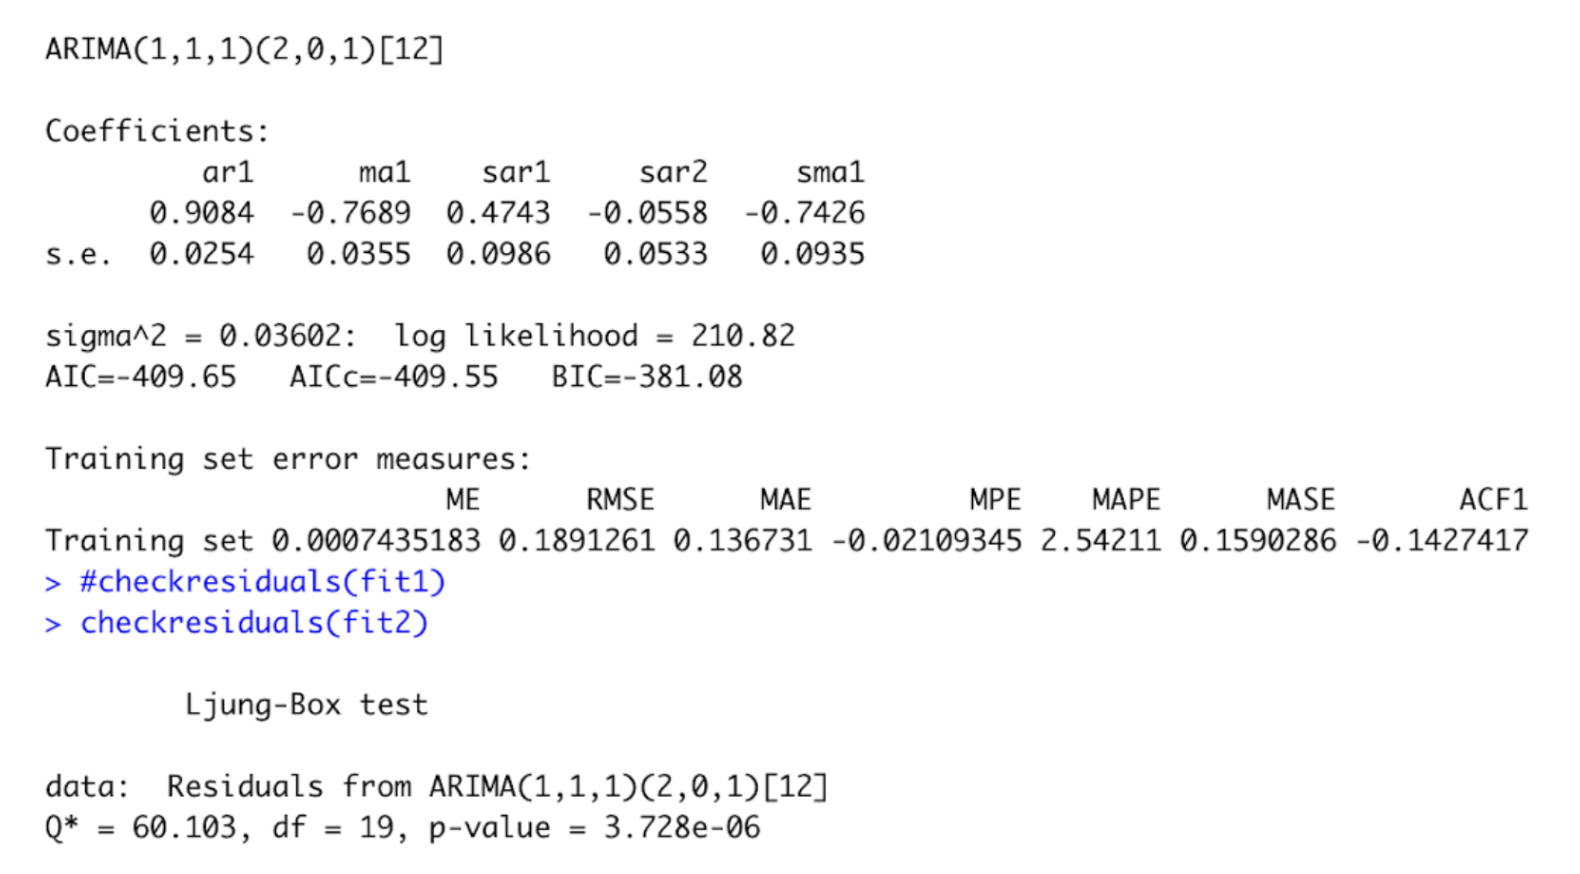
\includegraphics[width=1\textwidth]{assets/arima.png}
			\textit{Figure 2}
		\end{center}

		ARIMA function uses 3 parameters p,d and q: p as the lag order, d as the degree of differencing needed for stationarity and q as the order of the moving average. We will use the set of (p,d,q) that yield the least error by the auto.arima() function defined in the forecast library. An alternative solution by-hand would be to use Auto Correlation Function (ACF) and Partial Auto Correlation Function (PACF) plots. Due to the large number of tools available, R is chosen over Python for the implementation of ARIMA. The RMSE for the model devised by ARIMA looks healthy with RMSE of 0.1891, which suggests simulated and observed data are close to each other. 
		
		\begin{center}
			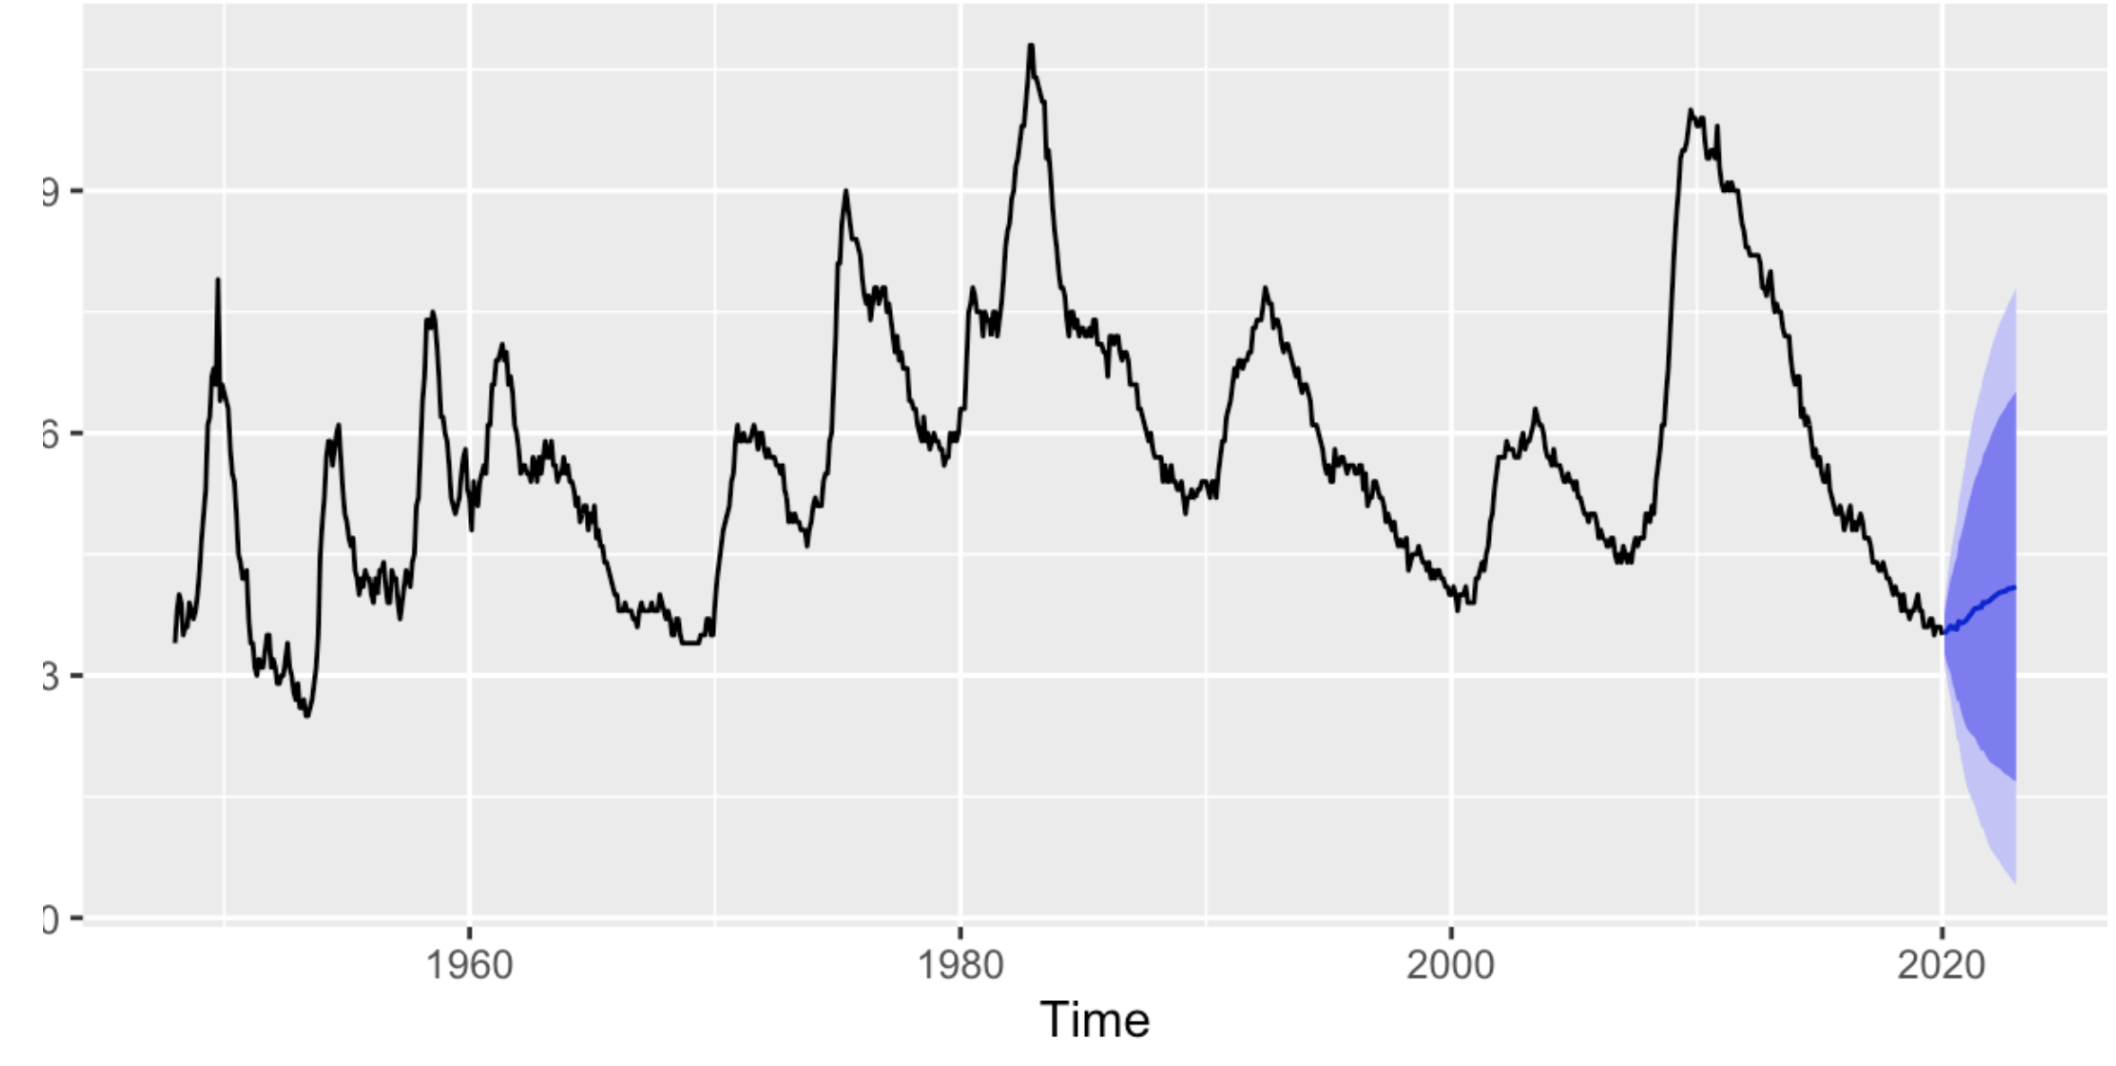
\includegraphics[width=1\textwidth]{assets/arima2.png}
			{Forecasts from ARIMA(1,1,1)(2,0,1) }
		\end{center}
		Since we haven’t included data past 2020, our forecast horizon for ARIMA was 42 months to get a view of the UR for the forthcoming 6 months:
		\begin{center}
			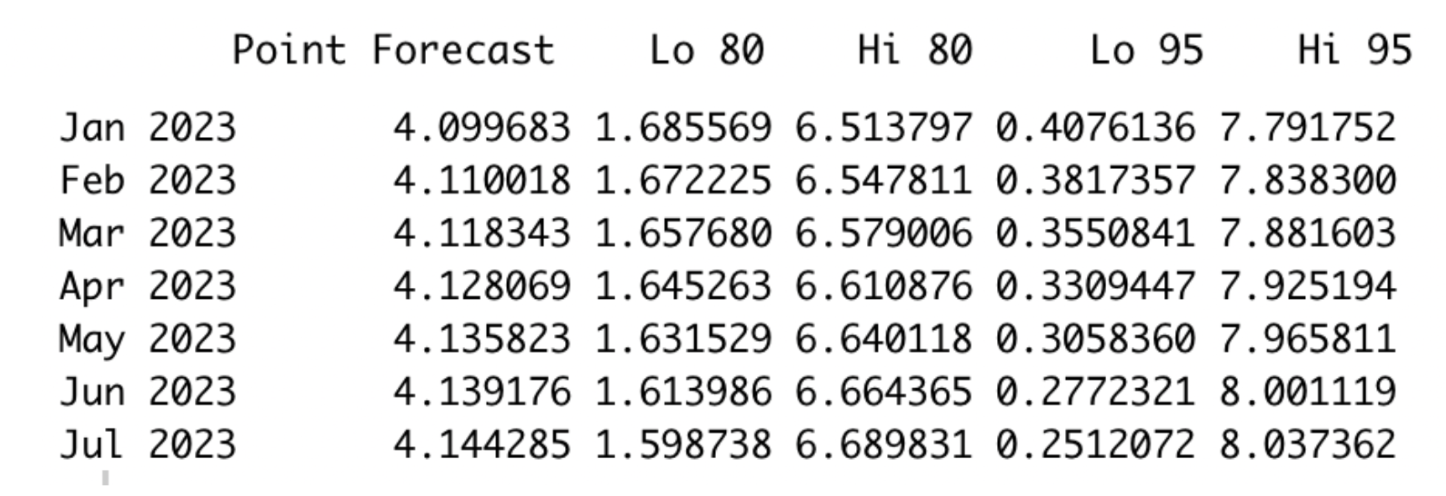
\includegraphics[width=1\textwidth]{assets/arima3.png}
			{Forecasts from ARIMA(1,1,1)(2,0,1) }
		\end{center}
	\subsection{Decision Tree}
	Decision Tree is a good tool for detecting patterns, classification and prediction. The Decision Tree model can help us to build the predictive model based on the training dataset (ex. 50% of the original dataset), and further assessed on the predictive ability of the model using testing dataset (50% of the original dataset). 
	Variables, such as food prices or inflation, are used to create splitting rules. The ones at the top of the tree would be considered the most important predictors, and variables included lower down in the tree are less related to the outcome. The outcome variable, which is the Unemployment Rate, can be classified as “High” and “Low” in the final decision node.
	This model would be very useful in presenting findings to people not knowledgeable in topics related to the UR, because of the simple logic for classifying and easy result to read. The entropy (e) and Information Gain (IG) are concepts that are useful when deciding the splitting order. Decision tree works by classifying information groups (nodes) with respect to orderliness, measured by entropy:
	
	\begin{equation}
		e= \sum_{i=1}^{K}(-P_{i} log_2 P_{i})
	\end{equation}
	The key element of the decision tree is the splitting nodes, that is defined by a variable and set of values it’s allowed to take. Information gain is the weighted change of entropy, and is the decisive factor in splitting the data.
	\begin{equation}
		IG =e_s - \sum_{i=1}^{K}(w_i e_i)
	\end{equation}
	Based on our decision tree model below, Rice price is the root node which indicates that it is the most important feature, and the UR data from Hungary, Hong Kong, and Australia were significant predictors as well. The RMSE of this model is 0.912.
	\begin{center}
		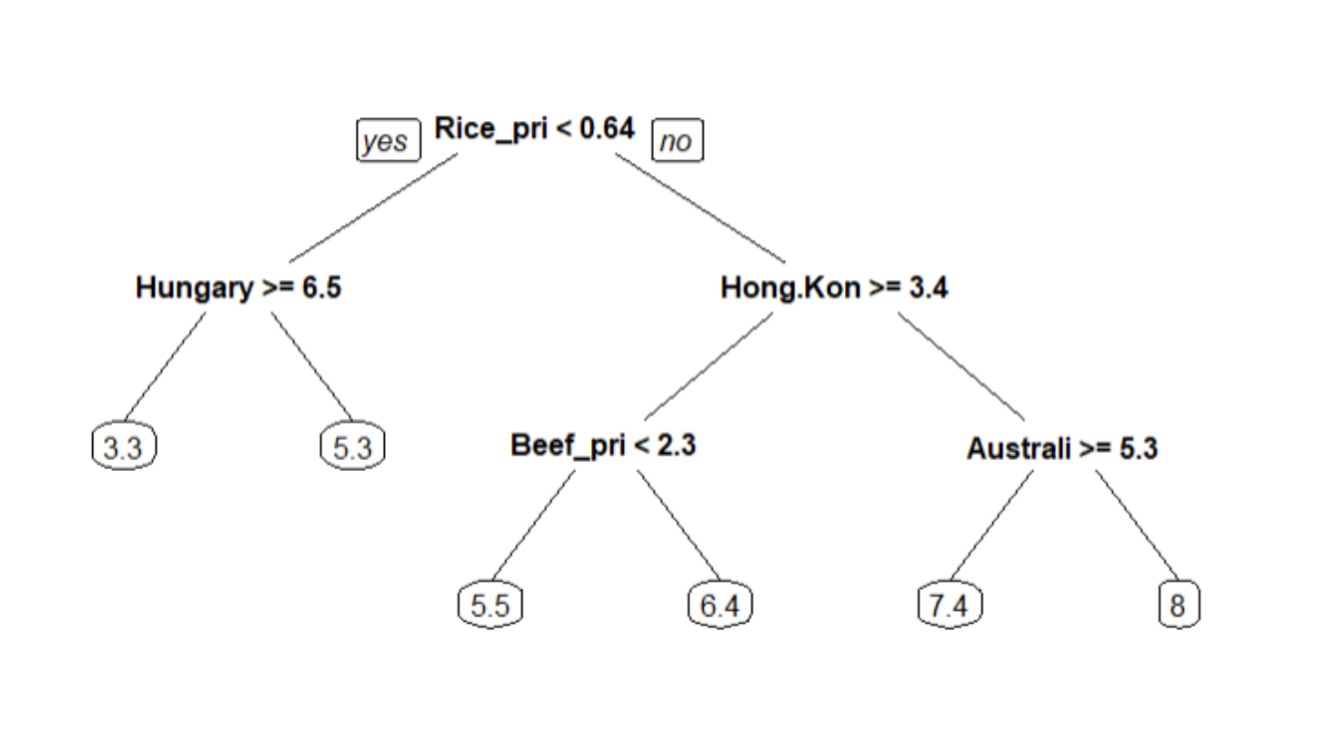
\includegraphics[width=1\textwidth]{assets/decisionTree.png}
		{Tree before pruning }
	\end{center}
	The performance of a decision tree can be improved by pruning. We have decided to use the prune function in order to remove the branches with less important features and reduce the complexity by using cross-validation with 10 folds. The decision tree below shows the tree after pruning. As a result, Beef price and UR data for Australia were removed. The RMSE of this model is 0.889, which only shows slight improvement from the previous decision tree. 
	\begin{center}
		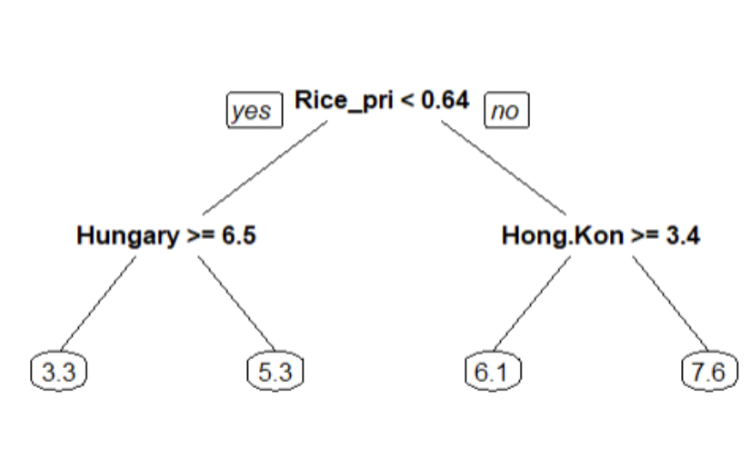
\includegraphics[width=1\textwidth]{assets/prunedTree.png}
		{Tree after pruning}
	\end{center}

	\subsection{Random Forest}
	Random forest is an algorithm that combines multiple decisions to create a “forest”, which can be used for both regression and classification. We will be using this method to find out the most important factors that affect the unemployment data in the U.S. and accurately forecast the UR.

	This method is used to make a prediction based on the average or mean of the output of various trees. It increases precision and accuracy, and reduces overfitting of the model. Thus, we expect it to perform better than the decision tree model we built. Using the same combined dataset with macro data, UR of other countries, and retail food prices, we can train a model and check its performance. It is also essential to choose the right tree size to include in the model, and we chose a Ranger function to tune the model and perform a larger grind search across several hyperparameters [6].
	
	The summary of a Random forest regression model evaluation with the initial set of hyperparameters, with RMSE = 0.4122 is shown below.
	\begin{center}
		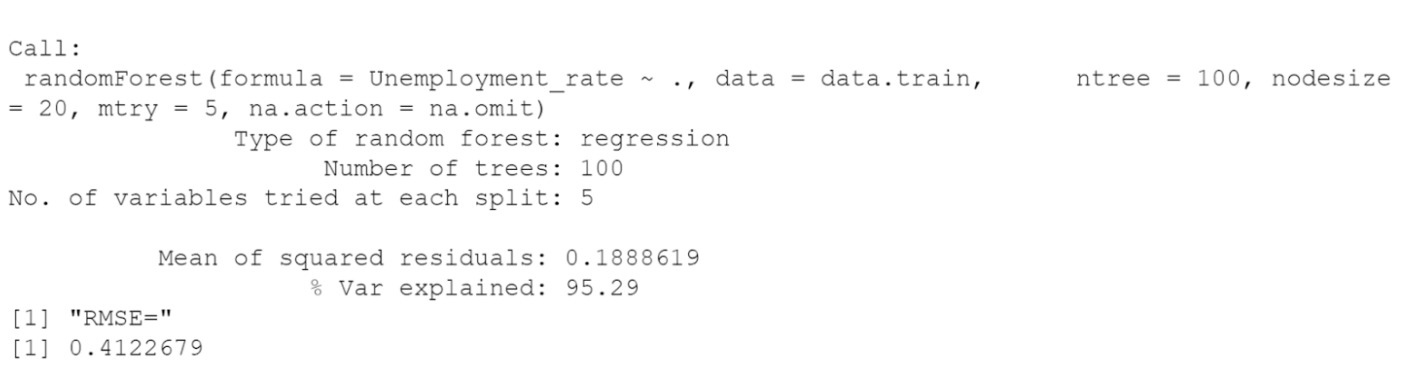
\includegraphics[width=1\textwidth]{assets/rf.png}
		{Model Summary}
	\end{center}
	This model can definitely be improved by changing parameters, so the grind search has been performed to evaluate which set gives the lower RMSE:
	\begin{center}
		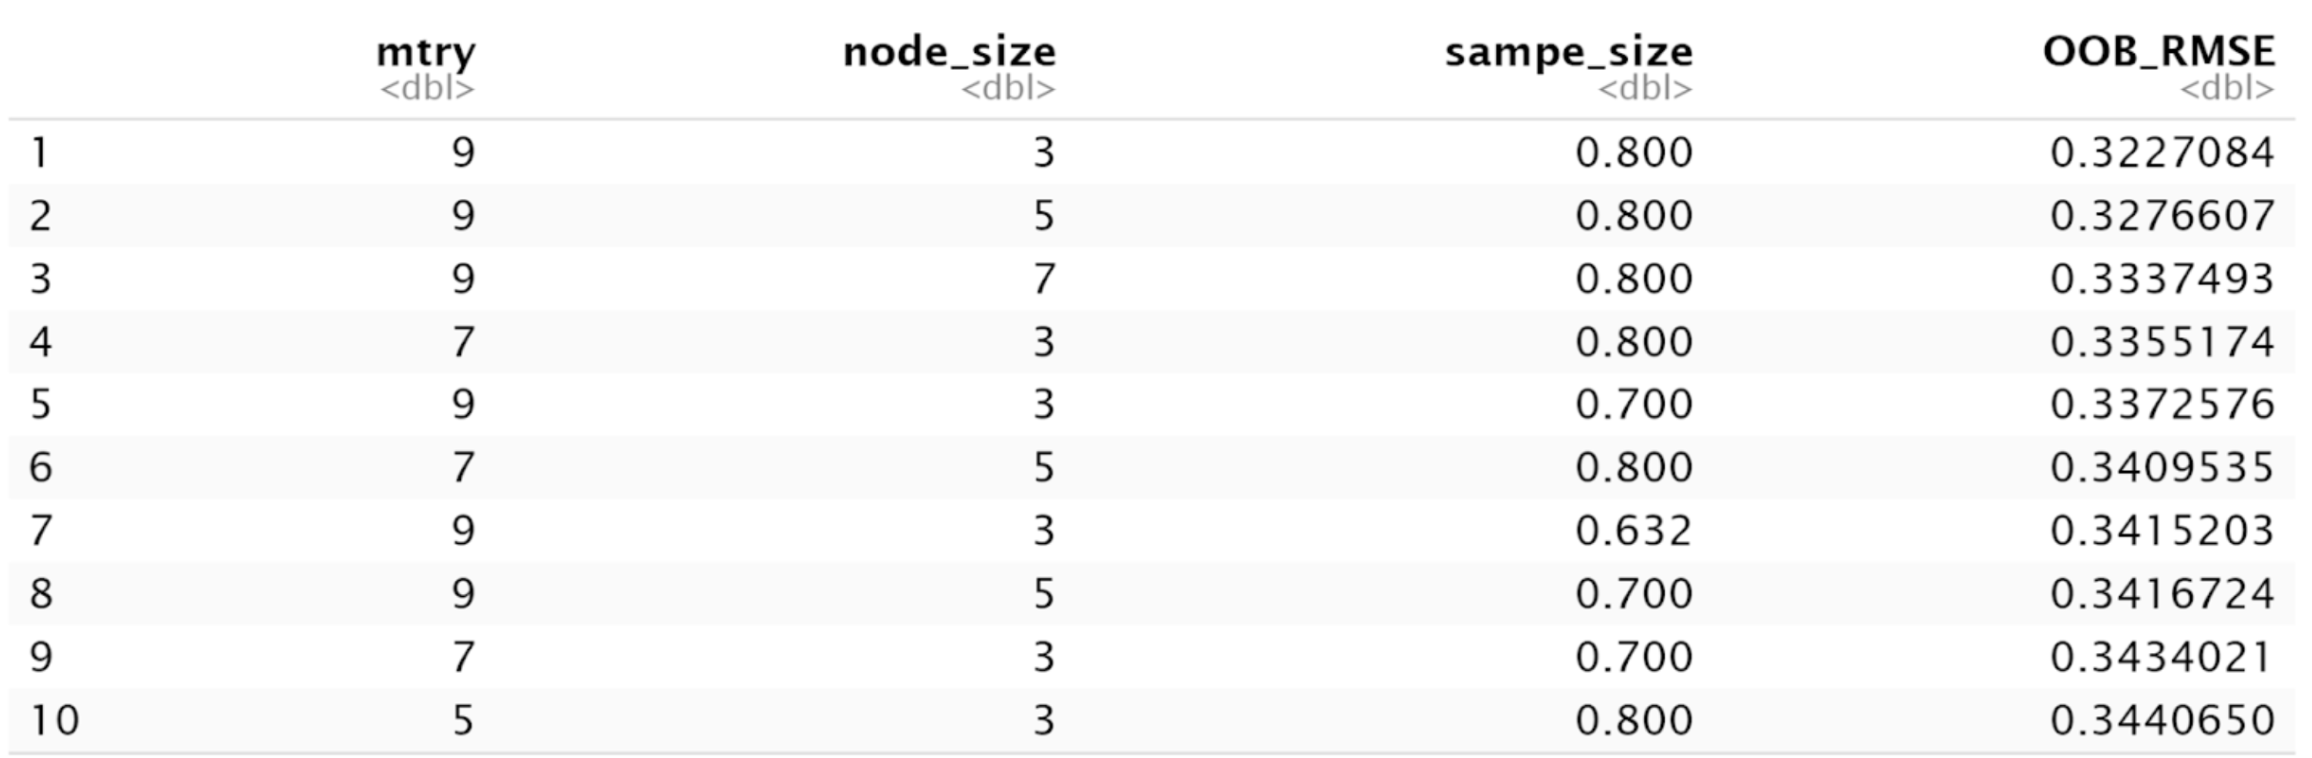
\includegraphics[width=1\textwidth]{assets/rfTable.png}
		{Evaluation of Alternatives}
	\end{center}
	According to the results of the evaluation, we should choose ntrees = 500, mtry = 9,  and nodesize = 3, and get a model with lower RMSE:
	\begin{center}
		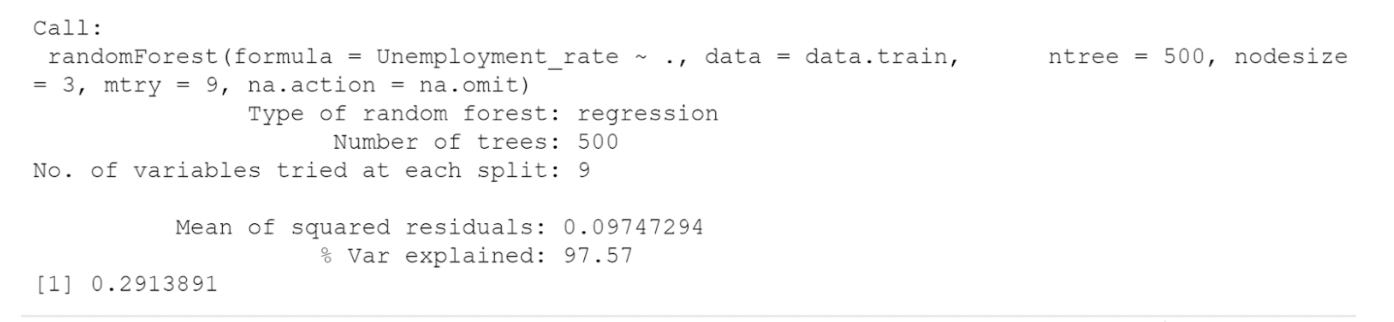
\includegraphics[width=1\textwidth]{assets/bestRf.png}
		{Best Model Summary}
	\end{center}
	New RMSE of this model is 0.291, which is still higher than ARIMA RMSE, and thus, we are not using a Random Forest model for making a prediction of the unemployment rate in the US in 2023.


\section{Results}
Comparison of method alternatives will be conducted using Root Mean Squared Error values for the proposed models. The lowest RMSE result indicates the most accurate model on past values, thus is assumed to yield the most accurate forecast. For this reason, there is no need to forecast UR using other methods.

\begin{center}
	\begin{tabular}{ |p{3cm}||p{3cm}||p{3cm}| }
		\hline
		\multicolumn{3}{|c|}{Comparison Table} \\
		\hline
		Method Name& RMSE Value &June'23 Forecast\\
		\hline
		Linear Regression  & 0.5543    &-\\
		ARIMA&   0.189  &  \%4.10 \\
		Decision Tree &0.889 & -\\
		Random Forest    &0.291 & -\\
		\hline
	\end{tabular}	
\end{center}


\section{Discussion}

	\subsection{Conclusion}
	Given the RMSE Plots for methods explained in sections between 2.1 and 2.4, We conclude ARIMA has the lowest RMSE for its model, thus will yield the most accurate forecast of UR. ARIMA has drawbacks stated by many researchers for neglecting the explanatory variables and conducting the forecast solely on the past values [5]. Forecasting the unemployment rate is extremely difficult and demanding with many inherent uncertainties. Indeed, the findings, when accurate, are helpful for many industry executives and employees for planning purposes. 
	
	\subsection{Limitations}
	The methods employed in this paper are completely algorithmic, meaning that no human input affects the forecast result. The obvious advantage of this approach is that the process is completely autonomous and trustless, meaning that trust in a third-party is not required for a forecast (such as the case in a forecast conducted by FED). It’s important to note the tradeoff for this advantage, which is the incapability to include rapid changes in monetary policy, pandemics, natural disasters and such.  An interesting continuation of machine-learning work presented in this paper would be a comparison of neural networks and deep-learning networks. Picking the best methods for forecast in each category and comparing the least wrong out of the three will provide a rather holistic view of which family of models works best for forecasting UR.


\section{Appendix}

\subsection{Residuals for Linear Regression}
	\begin{center}
		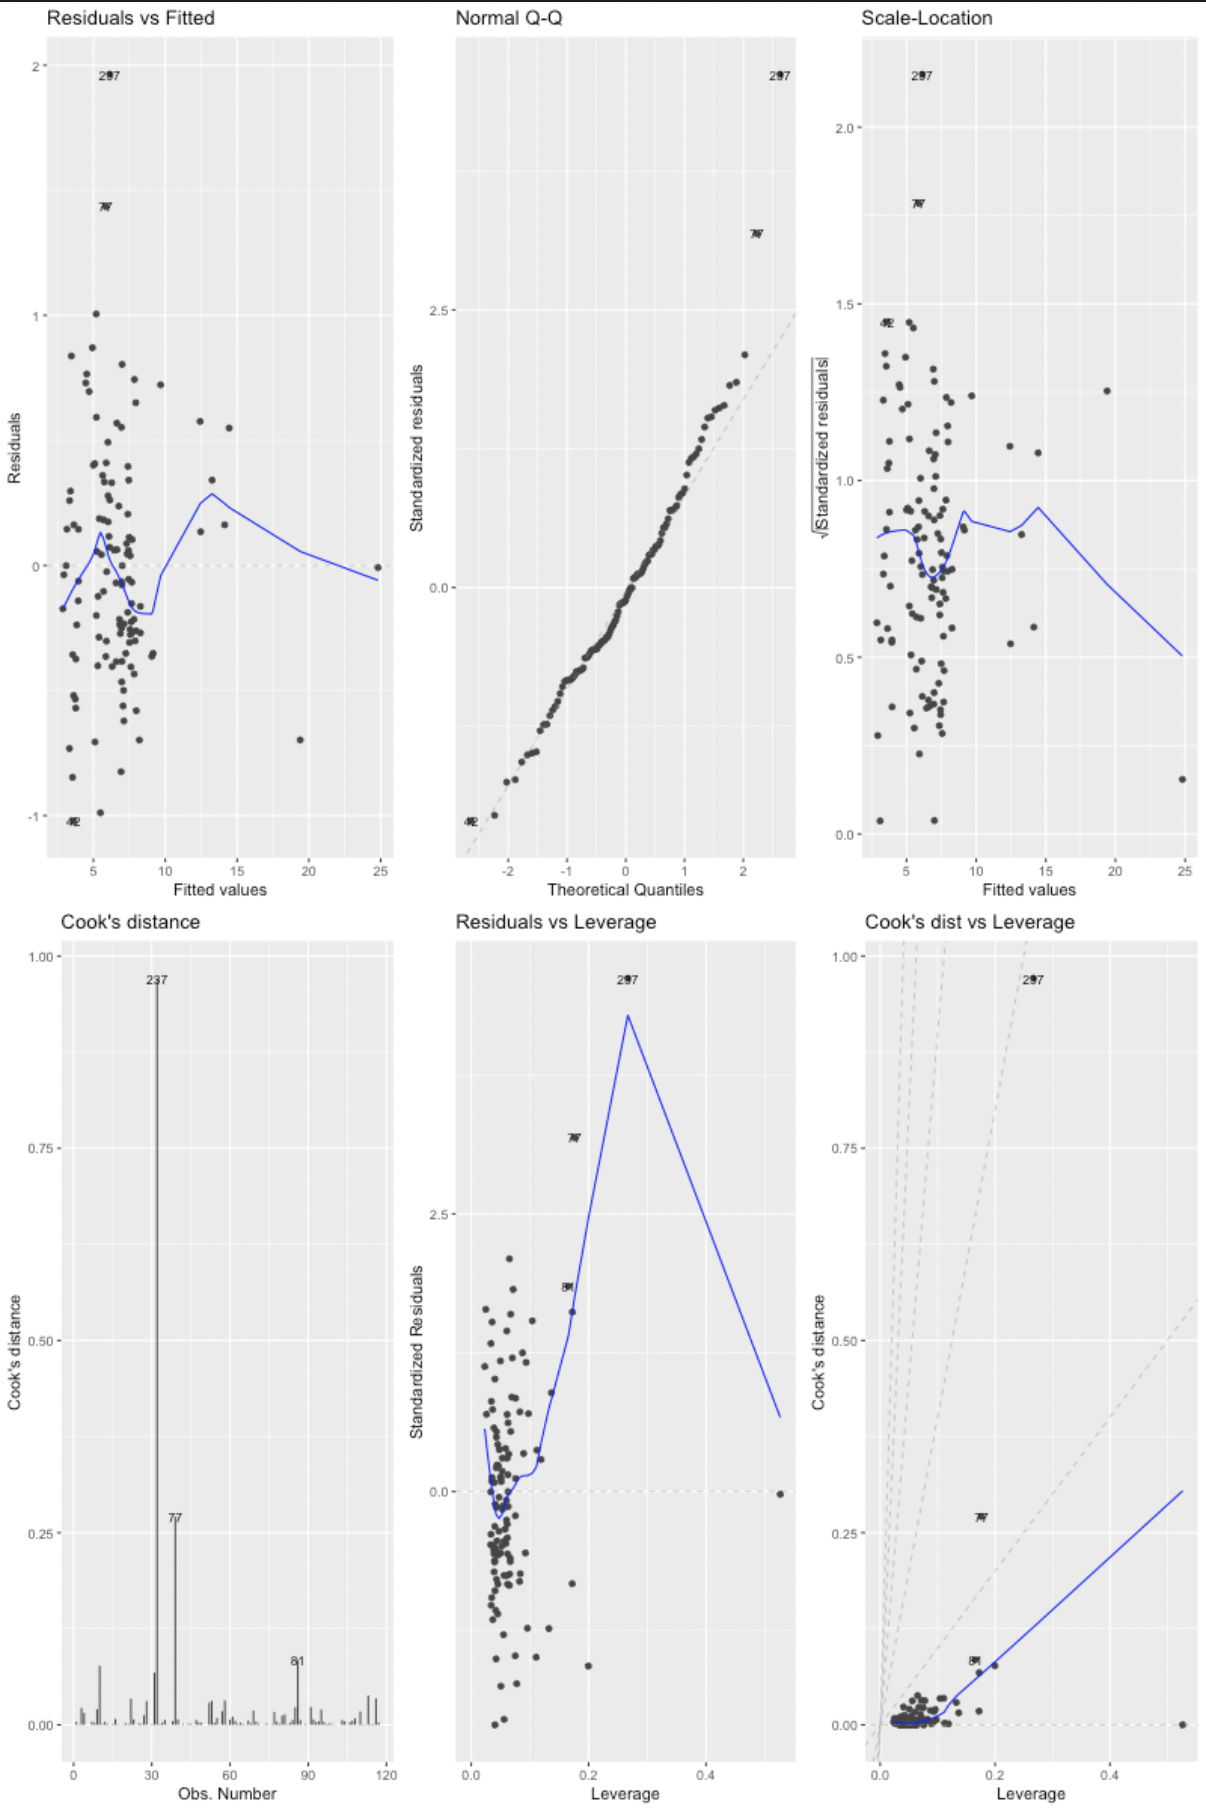
\includegraphics[width=1\textwidth]{assets/residual1.png}
	\end{center}
	\subsection{Residuals for ARIMA}
	\begin{center}
		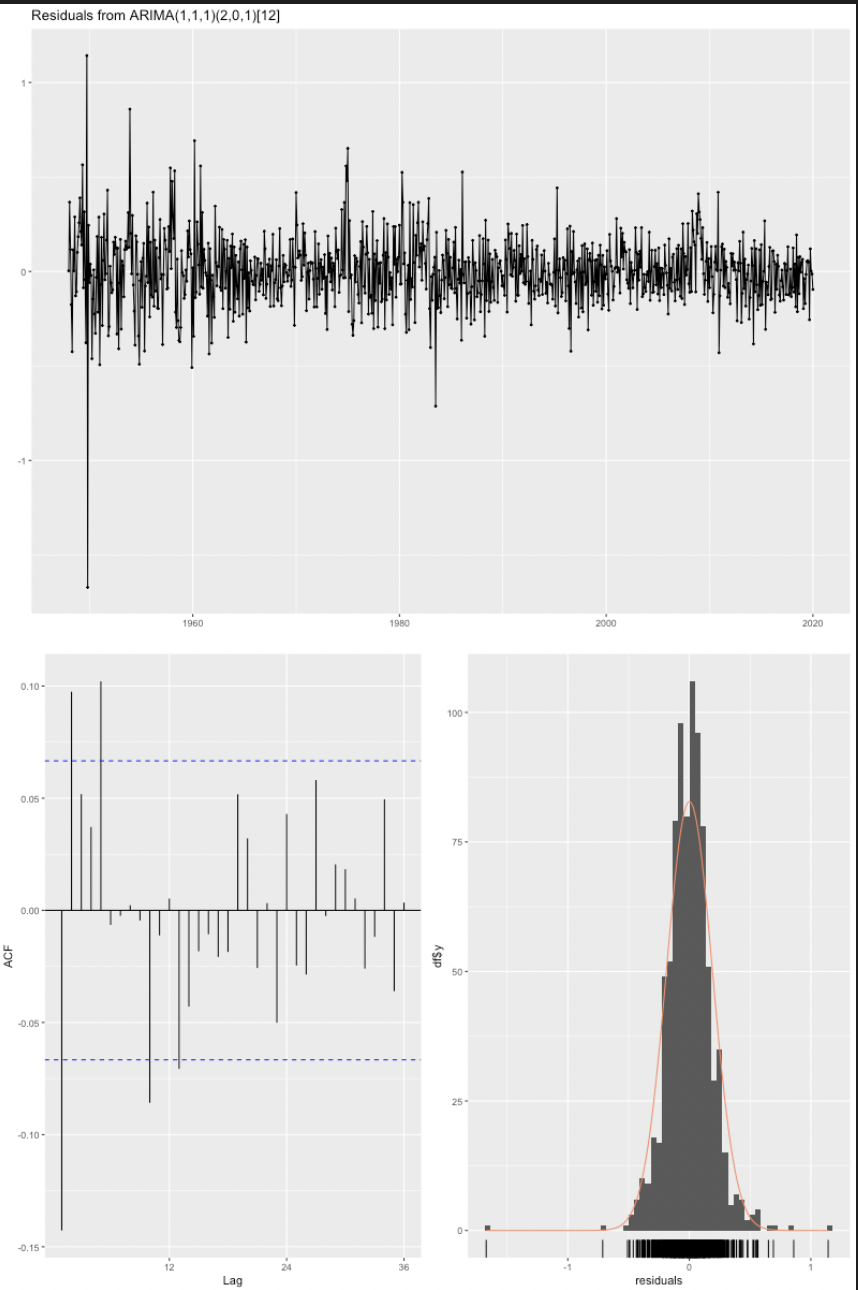
\includegraphics[width=1\textwidth]{assets/residual2.png}
	\end{center}
\subsection{Residuals for Decision Tree}
	\begin{center}
		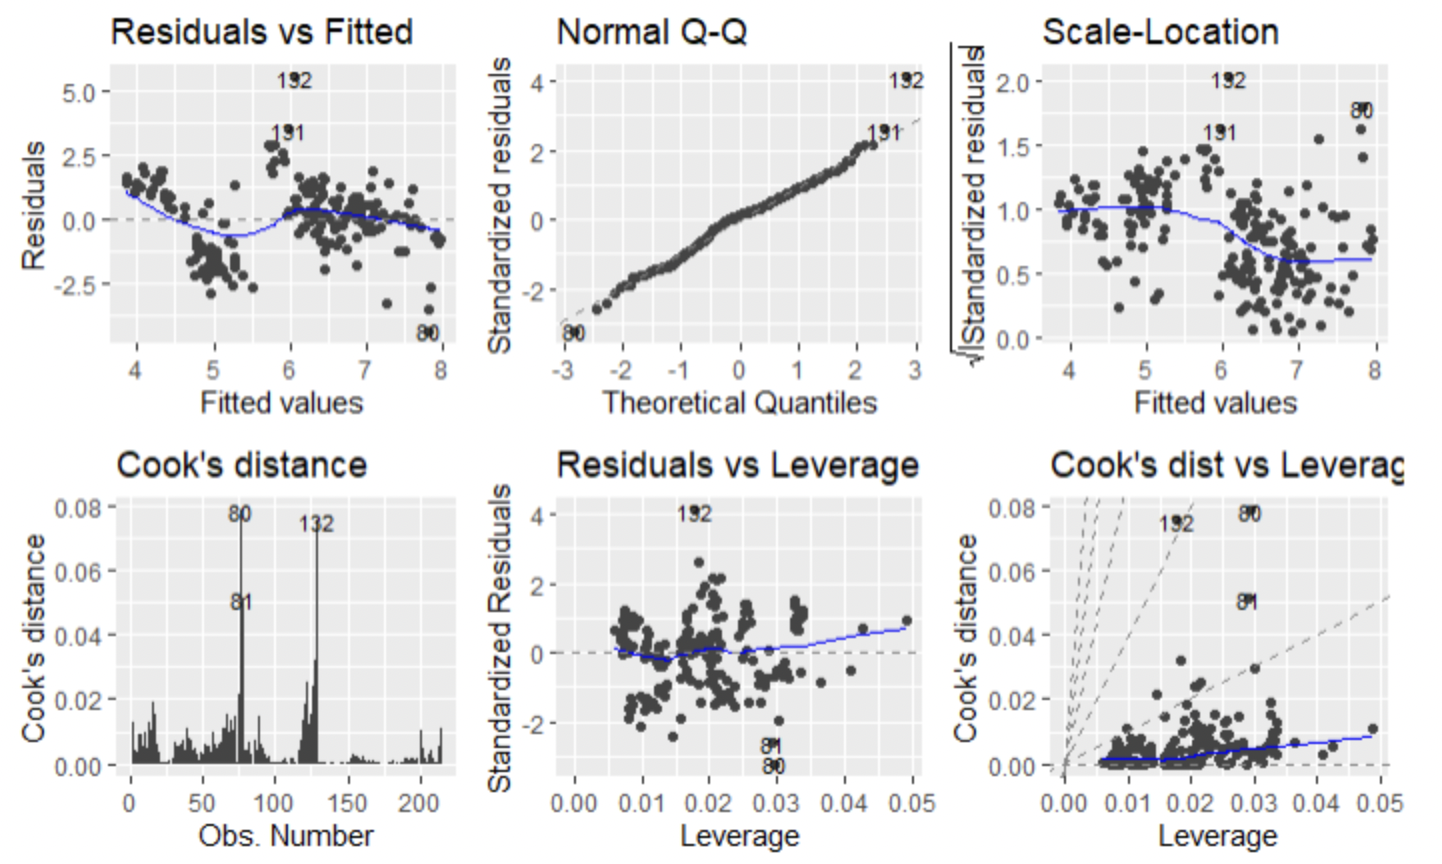
\includegraphics[width=1\textwidth]{assets/residual3.png}
	\end{center}
\subsection{Residuals for Random Forest}
	\begin{center}
		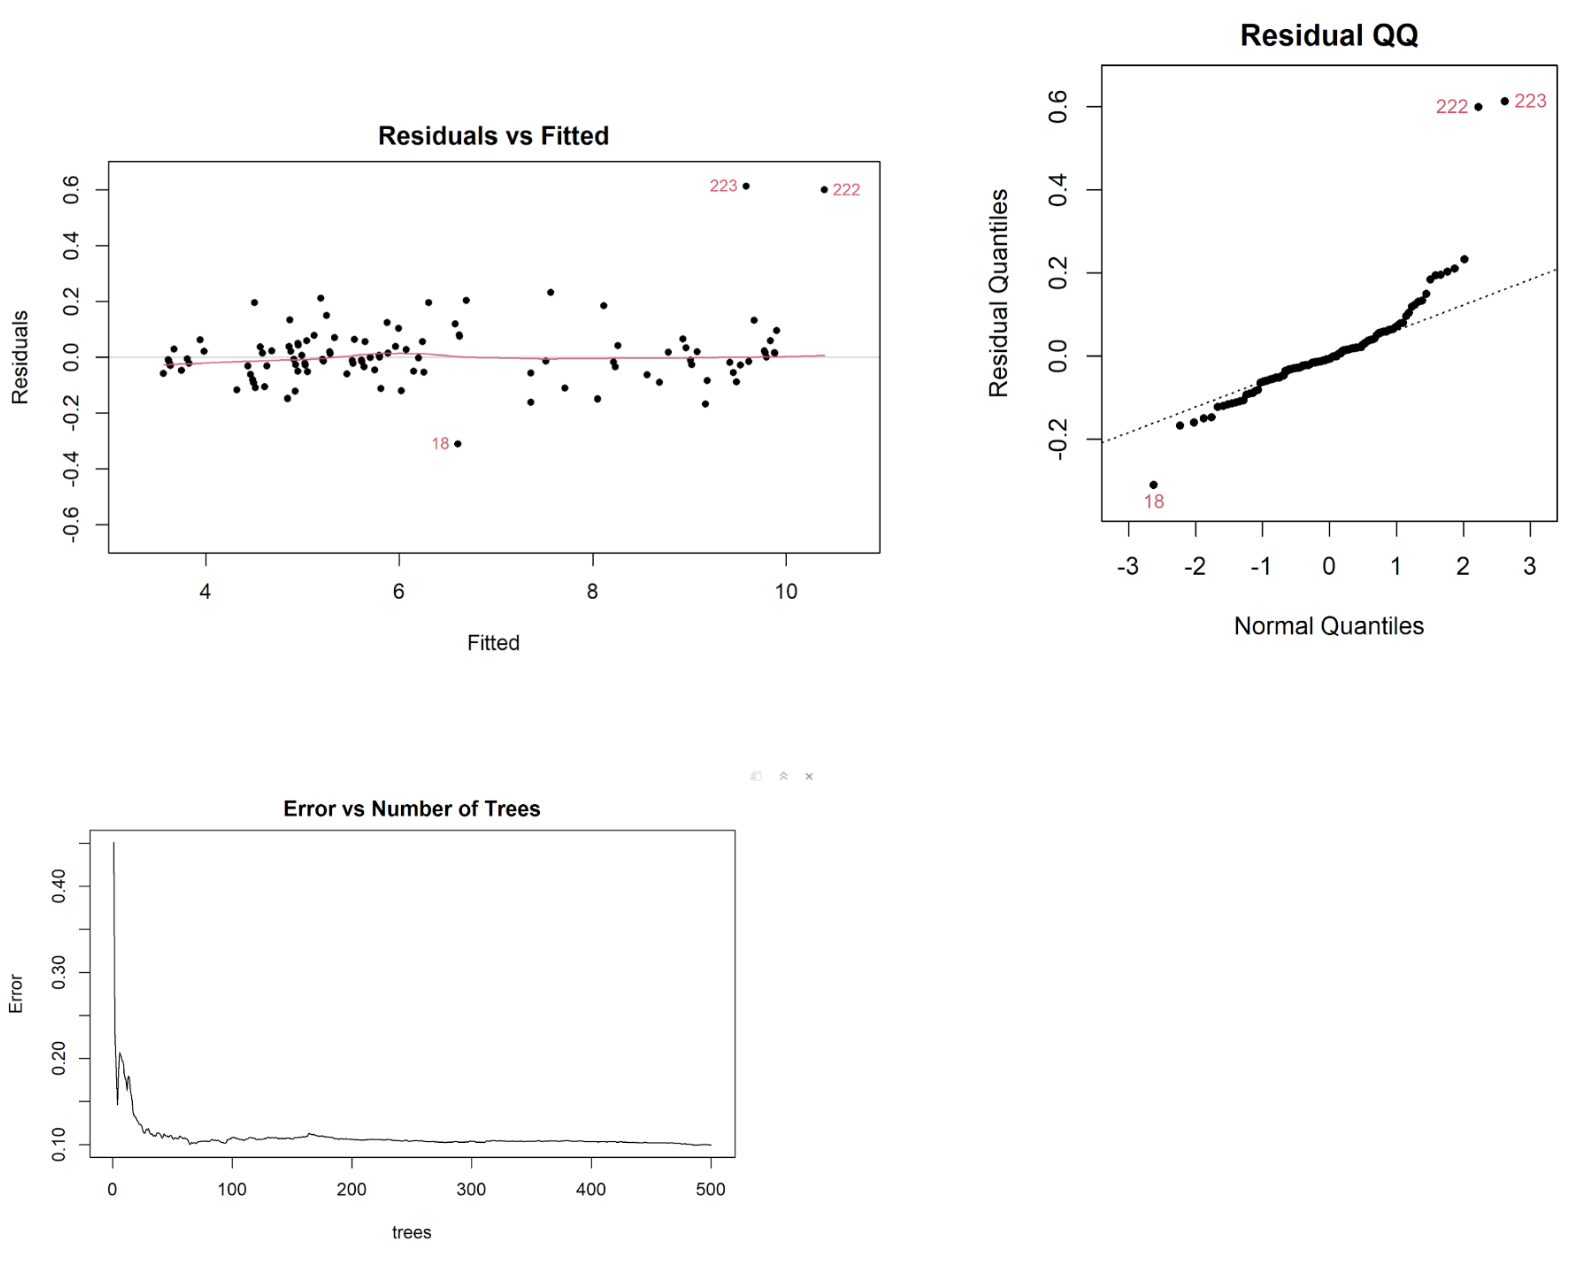
\includegraphics[width=1\textwidth]{assets/residual4.png}
	\end{center}

	\section{References}
		\begin{enumerate}
			\item Gostkowski, Michał, and Tomasz Rokicki. “Forecasting the Unemployment Rate: Application of Selected Prediction ...” Researchgate. Accessed December 13, 2022.
			\item U.S. Bureau of Labor Statistics. “Unemployment Rate.” Stlouisfed.org, 2022, \newline fred.stlouisfed.org/series/UNRATE.
			\item Phillips, A. W. “The Relation between Unemployment and the Rate of Change of Money Wage Rates in the United Kingdom, 1861-19571.” Economica, vol. 25, no. 100, Nov. 1958, pp. 283–299, 10.1111/j.1468-0335.1958.tb00003.x.
			\item Bernard, Andrew B., and Steven N. Durlauf. “Interpreting Tests of the Convergence Hypothesis.” Journal of Econometrics 71, no. 1-2 (March 1996): 161–73. https://doi.org/10.1016/0304-4076(94)01699-2.
			\item Nikolaos, D., Stergios, A., Tasos, S., \& Ioannis, S. (2018). Forecasting Unemployment Rates in Greece. International Journal of Sciences: Basic and Applied Research (IJSBAR), 37(1), 43–55.
		\end{enumerate}


\end{document}